\chapter{Continuous Integration and Continuous Delivery} \label{ch:cicd}

This notebook is mainly about Linux. In this appendix chapter, the boundary of the notebook is slightly expanded to software development, which is very often what Linux is used for in practice. \mync{Continuous Integration and Continuous Delivery}[CI/CD] is a widely accepted concept and philosophy in nowadays software development. This chapter introduces CI/CD as well as tools to carry out CI/CD.

Git and GitHub has been introduced in Chapter \ref{ch:git}. Git is a very useful software management tool in CI/CD, and GitHub one of the most widely used platforms that provides CI/CD relevant services. This appendix chapter is an extension to Chapter \ref{ch:git} where more about Git and GitHub are introduced from CI/CD perspective.

Some contents of this chapter come from \cite{honai2023cicd}.

\section{Agile VS Waterfall}

Agile and waterfall are both project management methodologies. Both of them are introduced here, starting with the more conventional waterfall model, and then Agile.

\subsection{Waterfall}

Speaking of project proposal, development, testing and delivery cycle, it is fairly intuitive to follow the procedures below:
\begin{enumerate}
	\item Understand requirements from the user.
	\item Design the architecture of the solution.
	\item Develop the solution.
	\item Test the solution.
	\item Deliver the solution and close the project.
	\item (Follow-up) maintain the solution.
\end{enumerate}
The philosophy behind waterfall, as its name indicates, is to ``follow the procedures and do not turn back''. When a previous step is considered completed, it is completed and should not be revoked or revised. This is demonstrated by Fig. \ref{ch:cicd:fig:waterfall}.
\begin{figure}[htbp]
	\centering
	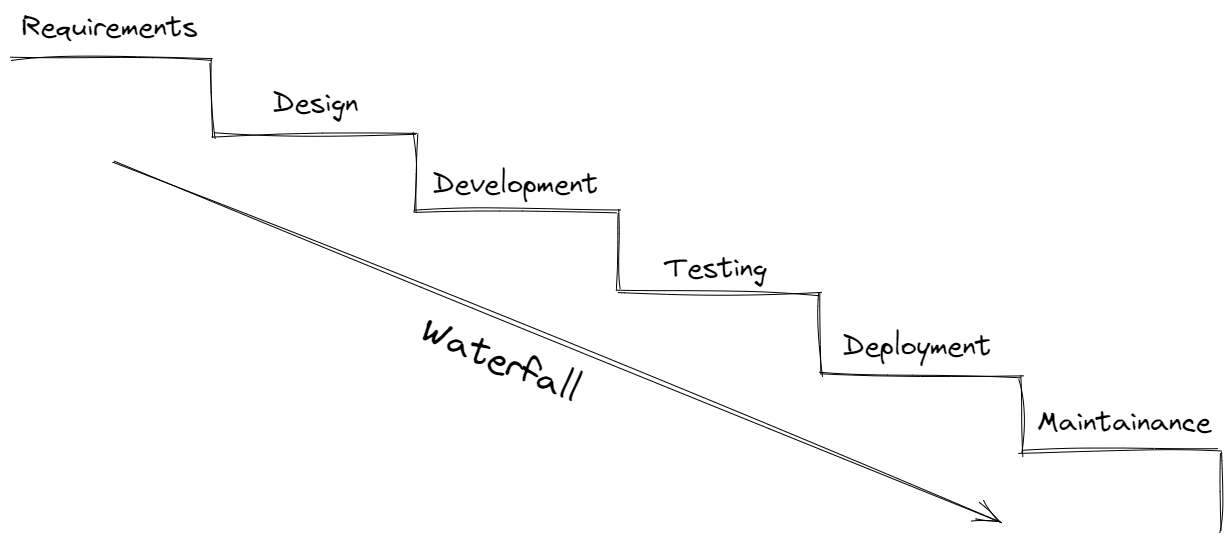
\includegraphics[width=300pt]{chapters/ap/figures/waterfall.png}
	\caption{Waterfall model.} \label{ch:cicd:fig:waterfall}
\end{figure}

With waterfall, a project can be designed, developed and deployed in a relatively efficient manner. However, there is one limitation: everything done in earlier steps cannot be changed in later steps. This sets up a high bar on both the user and the developer. For example, in step 1 ``understand requirements from the user'', the user needs to illustrate all the requirements to the developer as they cannot be modified in later steps. Similarly, in step 2 ``design the architecture'', the developer needs to optimize the design to his best, as the architecture cannot be changed later.

Regrettably, with the rapid change in the market and the aggressive advent in technology today, it is challenging even for the smartest users and developers to determine all the requirements and designs in the beginning stage of the project. More likely, the requirements of the user have to change to adapt to the market trend, and so does the technologies used in the solution.

For a new feature to be added into the existing system, it is possible to simply start a new project flow for the new feature, and integrate it into the existing system later. However, integrating the new feature into the existing system can also be challenging when the design is complicated and coupled. The integration often introduces a blackout period of the system. If the system is already deployed, the customer experience would be affected by the blackout.

\subsection{Agile}

Agile is the counterpart of waterfall. It is proposed to tackle the aforementioned issues: rapid change of requirements and adaptations to new technologies and tools. It allows continuous integration and delivery of new features into the system in a convenient and consistent manner without introducing blackout.

In agile architecture, each feature is separately modularized. Each feature, before deploying and integrating into the production environment, circulates in its own ``development and testing circle'', where it can be tested and reviewed iteratively by the developers and the users audit team, as shown in Fig. \ref{ch:cicd:fig:agile}.
\begin{figure}[!htb]
	\centering
	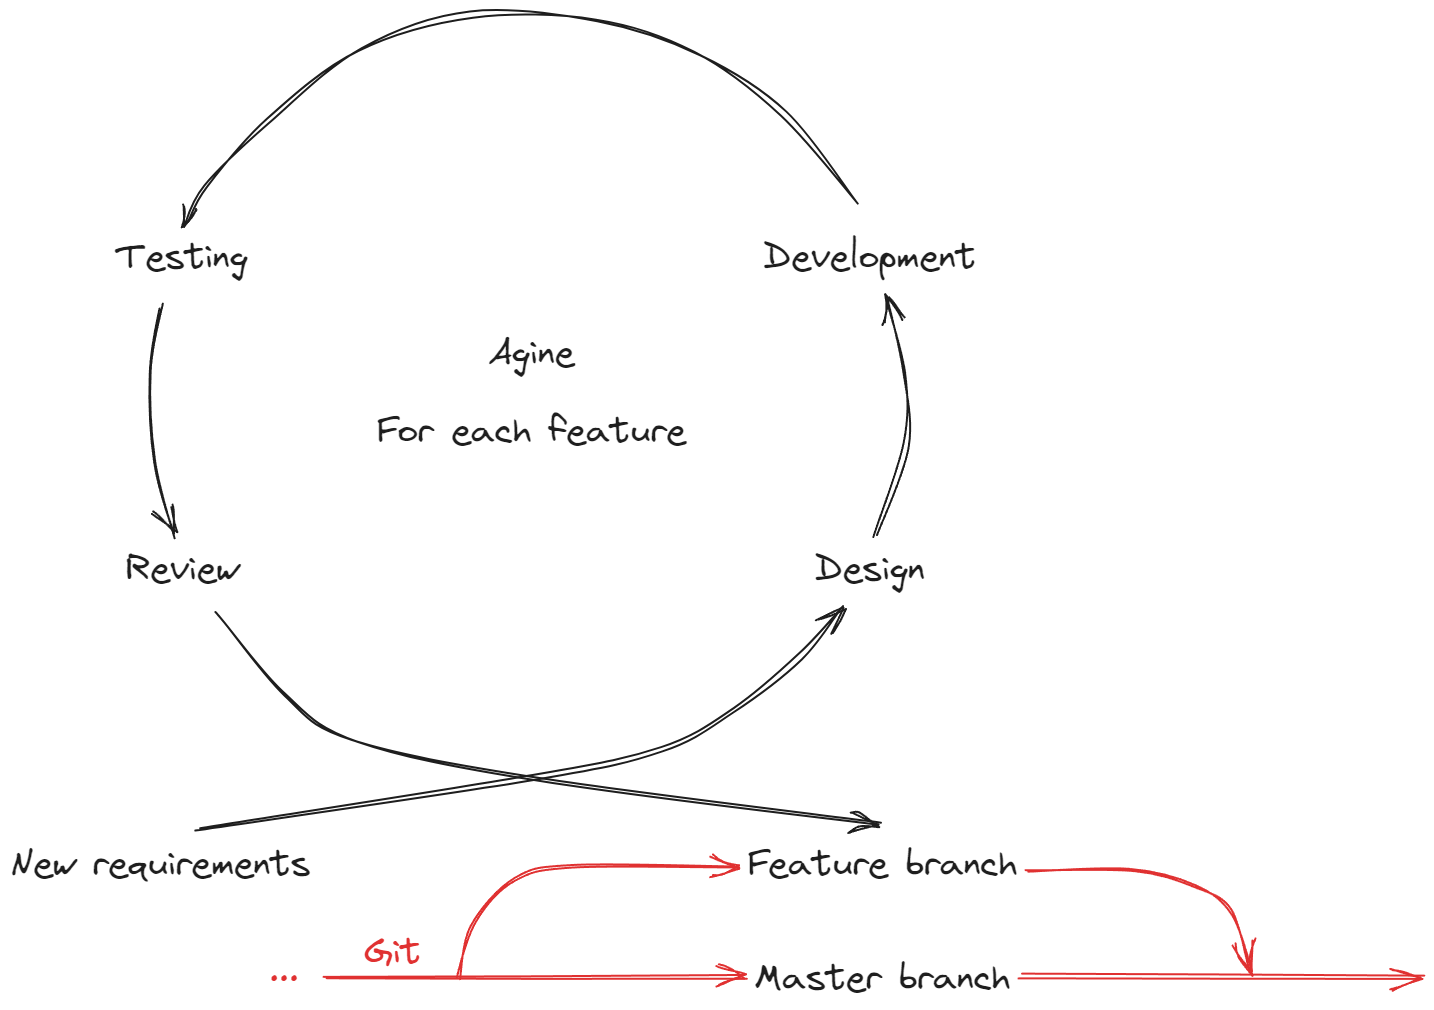
\includegraphics[width=300pt]{chapters/ap/figures/agile.png}
	\caption{Agile model.} \label{ch:cicd:fig:agile}
\end{figure}

Agile allows rapid change to be made to the requirements and realizations of a feature. Should there be a change, just keep cycling in Fig. \ref{ch:cicd:fig:agile} until the change is implemented and tested, before it is pushed back to the master branch.

In parallel development where there are multiple features running in their associated circles, the developer can easily choose which feature branch and circles to prioritize. This gives the developer a clearer overview of what is happening and how to best response to the customers immediate requirements.

As will be introduced later, agile is widely used in CI/CD.

\subsection{Roles in Agile-based Development}

Many roles are defined in the agile framework, each role coming with a responsibility. The roles may slightly differ for different projects. The most commonly seen set of roles known as \mync{scrum} is introduced in Table. \ref{ch:cicd:tab:agilerole}.
\begin{table}[!htb]
	\centering
	\caption{Roles in Agile model.} \label{ch:cicd:tab:agilerole}
	\begin{tabularx}{\textwidth}{lX}
		\hline
		Role & Description \\
		\hline
		Product owner & Manage the entire program. He understands all the user requirements and tracks the progresses of all the features under development. He signs off features before they are deployed. \\ \hdashline
		Scrum master & Lead the developer team as team manager or chief developer. He assigns tasks to the developer. \\ \hdashline
		Developer & Based on requirements, program the features. \\ \hdashline
		Tester & Design test cases to verify the efficacy of the developed feature. \\ \hdashline
		Operator/Supporter & Maintain the software in the production environment. \\
		\hline
	\end{tabularx}
\end{table}

In this role assignment, the product owner and scrum master come up with the product backlog, which clarify the sprints (tasks) and their priorities. The team then knows which sprints they shall work on first.

In the case where the features concern a professional domain (such as economics, medical, etc.) that the developers do not understand, business analysts are involved who bridge the user and the developer.

For each sprint, sprint planning and sprint backlog are proposed that describes the schedule of the sprint. The team works on the sprint and host daily scrum meetings until the sprint is solved. Upon finishing of a sprint, sprint review is hosted for audition.

\section{CI/CD Workflow}

CI/CD is both a philosophical concept and a bunch of technologies that speeds up the development, testing and deployment cycle of a software. It has become a common and beneficial practice for collaborative projects with rapid updates.

\subsection{Pipeline}

A \mync{CI/CD pipeline} refers to the procedure a task must go through before it is delivered to the production environment. It often involves the following steps:
\begin{enumerate}
  \item Integration
  \begin{enumerate}
    \item Commit and build the branch with the new features.
    \item Test the branch.
    \item Merge the branch with the master branch.
  \end{enumerate}
  \item Delivery
  \begin{enumerate}
    \item Release the master branch to the main repository.
    \item Deploy the solution to the production environment.
  \end{enumerate}
\end{enumerate}

\subsection{Continuous Integration}

In the development of a sprint, new codes are rapidly developed, and they are rapidly built, merged and tested.

Conventionally, the integration of a new feature requires involvement from multiple parties. An example is given in Fig. \ref{ch:cicd:fig:conventionalintegration}. It includes the developer who program the software following users (or business analysts) requests, the integration team who integrates the new feature with the existing system and compile the code into packages, and the operations team who upload the new system into the pre-prod environment for real data testing, and the testers who audit the output of the program running in the pre-prod environment.

\begin{figure}[!htb]
	\centering
	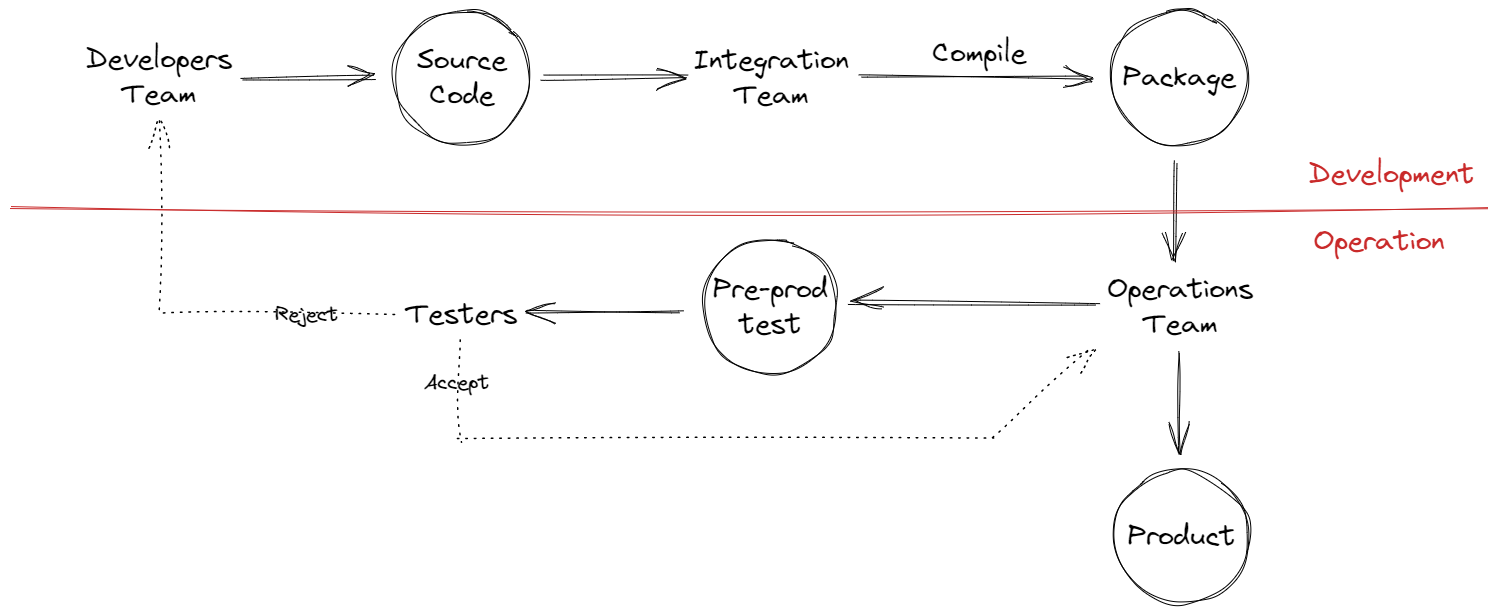
\includegraphics[width=350pt]{chapters/ap/figures/conventionalintegration.png}
	\caption{Integration and delivery of a new feature. The integration corresponds with the development and delivery, operation, in the figure respectively.} \label{ch:cicd:fig:conventionalintegration}
\end{figure}

Should there be any error along the way, the code is roll back the developer team for trouble shooting. When the new system with the updated code survives pre-prod environment, it is then pushed to the production environment.


In practice, each cycle in Fig. \ref{ch:cicd:fig:conventionalintegration} can take a few days or even weeks as so many teams have to cooperate to make it happen. It takes time for the integration team to integrate different branches in the source code together, making sure that components from different branches function properly. When there is a defect, the flaws can be spotted only in the last stage of the iteration, i.e., testing. This practically disallows very frequent update of the system in response to the rapid changes in requirements.

\myabb{Continuous Integration}{CI} (together with \myabb{Continuous Delivery}{CD} which is introduced in the later section) tries to solve the above problems. CI automates the ``development'' portion in Fig. \ref{ch:cicd:fig:conventionalintegration}, while CD automates the ``operation'' portion.

To speed up the development of new features, CI mainly adopts the following methods.
\begin{itemize}
	\item Use Git to manage features. This simplifies the procedure of managing multiple under-development features and integrating them together. Integration is now managed by Git following developers' intention.
	\item Use a build server to automatically compile the code into ready-for-delivery packages. The scrum master and senior developers can access the server and monitor the progression. Should there be a compiling error, the developer is notified immediately.
	\item The code, after compiling, is immediately tested in the build server using pre-defined test cases. If the code fails the test cases, the developer is immediately notified.
\end{itemize}

CI effectively removed ``integration team'' from the picture. The integration related tasks are split into small pieces and processed by automation tools, feature integration by Git, and compiling by build server. During CI, the developer not only generates the codes, but also supervises Git and build server. Should there be any error, the developer is notified immediately by the automation tools.

CI speeds up the developing cycle, from the receiver receiving requests from the user, to the point they have new system in the package ready for pre-prod testing.

\subsection{Continuous Delivery}

The package received from the development side contains the latest version of the system where a new feature is integrated. It is, however, not certain at this point whether the new feature works properly and how the system would behave as a whole with this new feature. The sophisticated testing and deployment of the software features are done by the operations team.

Conventionally, operations team and the testers receive the updated package together with an instruction from the developers team. The instruction describes how the package shall be installed, and what test cases to use for auditing. The operations team and the testers need to understand the instructions, and configure the pre-prod environment accordingly for the testing. The testers then uses varieties of scenarios to test the performance of the software. Bugs, if any, are reported to the developers team. If no bugs are spotted, the testers notify the operation team to release the package into production environment.

There are some obvious drawbacks to the conventional approach. The developers team needs to give detailed and precise instruction to the operations team, and the developers may make mistakes or missing something in the instruction, especially regarding environment configuration. Besides, there are too many human interactions, which slow down the process and generates human error. The entire procedure usually take about a whole day.

CD is a software development practice that allows software to be released to production at any time. The idea behind CD is to deploy the code for testing automatically anytime CI provides a new package by adopting the following methods.
\begin{itemize}
  \item Use machine-readable instruction files for packages installation, and let the server virtualize the execution environment and install the packages automatically.
  \item Use machine-readable testing scripts, and let the server execute tests and analyze the results automatically.
  \item The aforementioned machine-readable instruction files and testing scripts are managed the same way as the source code by the developers.
\end{itemize}

Ideally, as soon as a version of packages is released by CI, CD can automatically have it deployed and tested, and return the testing results to CI without human interaction. This is shown by Fig. \ref{ch:cicd:fig:cd}. In this CI/CD implementation, the developer is playing a more comprehensive role than what is shown in Fig. \ref{ch:cicd:fig:conventionalintegration}.
\begin{figure}[htbp]
	\centering
	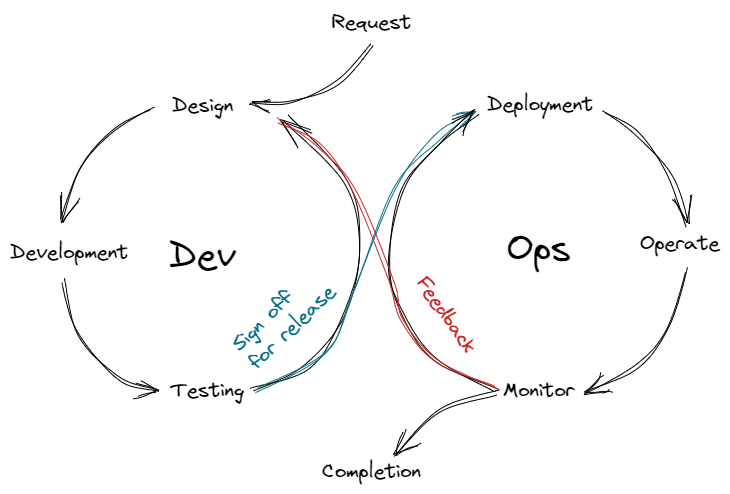
\includegraphics[width=350pt]{chapters/ap/figures/cd.png}
	\caption{CI and CD.} \label{ch:cicd:fig:cd}
\end{figure}

Under the framework of CI/CD in Fig. \ref{ch:cicd:fig:cd}, the developer not only develops the new feature, but also integrates the features with the help of version control and branch management tool Git, compiles the packages using build server, deploys the new packages in the testing environment by preparing machine-readable instruction files, and finally tests the new features using pre-configured test cases in the machine-readable testing scripts.

Since the operation team joins the developers team, they are now called the DevOps team. The CI/CD framework shown in Fig. \ref{ch:cicd:fig:cd} is known as the CI/CD pipeline which represents an end-to-end software development lifecycle (SDLC) within its ecosystem.

This CI/CD framework enables fast deployment of new packages. Large IT companies can make up to dozens of new releases everyday.

\section{GitHub Actions}

GitHub has been an amazing platform for managing software projects, especially open-source collaborative projects. In the early days when CI/CD was not enabled in GitHub, developers used third-party CI/CD tools such as Jenkins and Travis CI in conjunction with GitHub for fast and convenient integration and deployment. Lately, GitHub introduced \mync{GitHub Actions}, its own CI/CD solution, as a response to developers' requests.

GitHub Actions is essentially a workflow automation service that allows the user to define a sequence of actions that can be triggered by timers or repository-related events. The workflow can be used for both CI/CD tasks such as code building, testing and deployment, and for managing the repository such as adding labels. Machine-readable instruction files are used to configure the workflow and they are included in the repository and managed together with the source code.

This section gives a brief introduction to GitHub Actions. More details are given in \cite{git2025reference}.

\subsection{Workflow Building Blocks}

The basic building blocks of GitHub Actions include
\begin{itemize}
  \item Workflows
  \item Jobs
  \item Steps
\end{itemize}
A demonstrative plot is given in Fig. \ref{fig:actions_workflow}.
\begin{figure}[!htb]
	\centering
	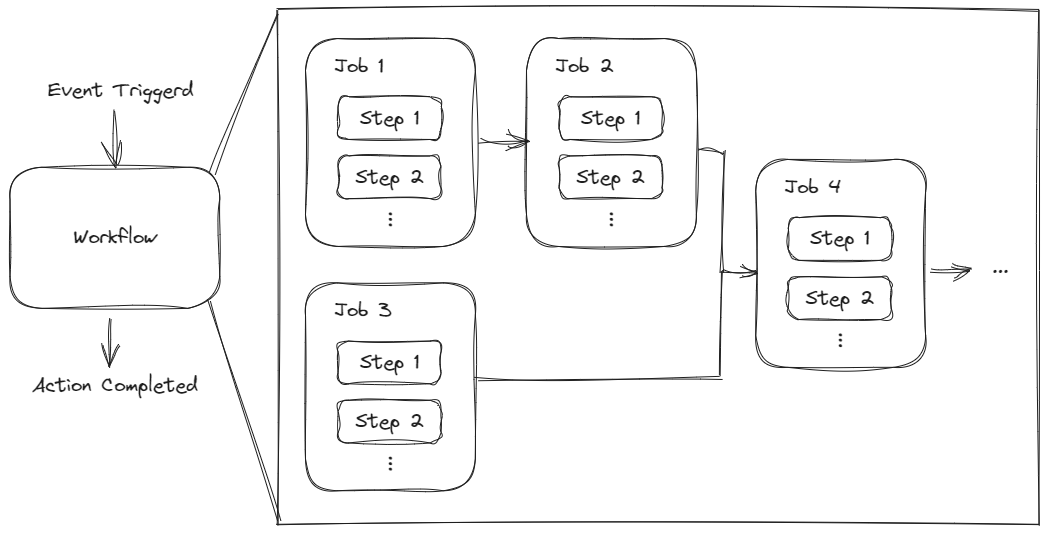
\includegraphics[width=350pt]{chapters/ap/figures/action_framework.png}
	\caption{A demonstration of GitHub Actions workflow.} \label{fig:actions_workflow}
\end{figure}

A workflow consists of jobs to be executed when a trigger happens. The jobs are executed in parallel by default (see ``job 1'' and ``job 3'' in Fig. \ref{fig:actions_workflow}), or in sequence when there are dependencies (see ``job 2'' and ``job 4'' in Fig. \ref{fig:actions_workflow}). Each job is executed in a dedicated VM or container known as a ``runner''. The running environment of a runner, such as OS, libraries, environment variables, etc., can be configured separately. In each job multiple steps can be defined. A step often corresponds with an action, such as executing a shell script. The steps in a job are executed in sequence in the configured order. Both steps and jobs can be triggered conditionally. There can be any number (at least 1) of steps in a job, any number (at least 1) of jobs in a workflow, and any number of workflows attached to a branch.

The user needs to formulate the pipelines to be executed automatically into GitHub Actions workflows.

\subsection{Supported Triggers}

It is worth mentioning that GitHub Actions can be triggered not only by repository-related events. Commonly seen triggers include
\begin{itemize}
	\item Repository-related events, such as push, pull request (most commonly seen).
	\item External events.
	\item Schedulers or timers.
	\item The user who triggers the workflow manually.
\end{itemize}

GitHub Actions provides workflow templates of different task types. There are at least the following workflow types as of this writing. They can be used for but not limited to CI/CD.
\begin{itemize}
	\item CI
	\item Deployment
	\item Testing
	\item Code quality
	\item Code review
	\item Dependency management
	\item Monitoring
	\item Automation
	\item Utilities
	\item Pages
	\item Hugo
\end{itemize}

A full list of GitHub events that can trigger GitHub Actions is given in \cite{git2025reference}.

\subsection{Jobs and Steps}

The workflows configuration files are YAML files that the user can either prepare from scratch or modify from existing templates on GitHub Marketplace, a platform where commonly used workflows are shared.

A workflow configuration file contains at least the following information:
\begin{itemize}
  \item The trigger of the workflow.
  \item The environment to execute the workflow.
  \item The actions in the workflow.
\end{itemize}

The YAML files should follow the syntax required by GitHub and be saved under \verb|.github/workflows/| so that GitHub is able to detect them as workflows and execute them accordingly.

An official demonstrative example of a GitHub workflow YAML file is given below \cite{git2025reference}. 

\begin{lstlisting}
name: GitHub Actions Demo
run-name: ${{ github.actor }} is testing out GitHub Actions
on: [push]
jobs:
  Explore-GitHub-Actions:
    runs-on: ubuntu-latest
	steps:
	  - run: echo "The job was automatically triggered by a ${{ github.event_name }} event."
	  - run: echo "This job is now running on a ${{ runner.os }} server hosted by GitHub!"
	  - run: echo "The name of your branch is ${{ github.ref }} and your repository is ${{ github.repository }}."
	  - name: Check out repository code
		uses: actions/checkout@v4
	  - run: echo "The ${{ github.repository }} repository has been cloned to the runner."
	  - run: echo "The workflow is now ready to test your code on the runner."
	  - name: List files in the repository
	    run: |
		ls ${{ github.workspace }}
	  - run: echo "This job's status is ${{ job.status }}."
\end{lstlisting}

Save the above YAML file under \verb|.github/workflows/| and GitHub would recognize the workflow. Click ``Actions'' on GitHub dashboard to check the details of the workflow.

A brief introduction to YAML file syntax for GitHub Actions is given below.

In the workflow of the demonstrative example only one job, namely ``Explore-GitHub-Actions'', is defined. In practice, multiple jobs can be defined in a workflow. An example from \cite{git2025reference} is given below where 3 jobs are defined.
\begin{lstlisting}
jobs:
  setup:
    runs-on: ubuntu-latest
    steps:
      - run: ./setup_server.sh
  build:
    needs: setup
    runs-on: ubuntu-latest
    steps:
      - run: ./build_server.sh
  test:
    needs: build
    runs-on: ubuntu-latest
    steps:
      - run: ./test_server.sh
\end{lstlisting}
Jobs are by default independent and can run in parallel unless \verb|needs| field is used just like in the above example, where ``build'' depends on ``setup'', and ``test'' on ``build''.

Commonly seen configurations in a workflow YAML file are given in Table \ref{tab:githubactions_workflow}.
\begin{table}[!htb]
	\centering \caption{Commonly seen configurations in GitHub Actions workflow.}\label{tab:githubactions_workflow}
	\begin{tabularx}{\textwidth}{lX}
		\hline
		Field & Description \\ \hline
		\texttt{name} & The static name of the workflow.  \\ 
		\texttt{run-name} & The name of an instance of run generated by the workflow.  \\ 
		\texttt{on} & The event(s) that triggers the workflow. A full list of supported events are given in \cite{git2025reference}. Multiple triggers are supported. The trigger can be configured very flexibly. \\ 
		\texttt{permissions} & Allowed r/w/x permissions for the workflow or for different triggers defined by the workflow. \\ 
		\texttt{env} & Environment variables to be used in the jobs descriptions. \\
		\texttt{defaults} & Default settings for all jobs. \\
        \texttt{concurrency} & Concurrency group of the workflow. There can be only one workflow running concurrently within a concurrency group. \\
        \texttt{jobs} & A dictionary of jobs. Each entry corresponds with a job. \\
		\hline
	\end{tabularx}
\end{table}

The \verb|jobs| field is a dictionary of jobs that run in parallel (unless \verb|needs| is used in the job description). Each entry in the dictionary corresponds with a job. The key of the entry is referred as \verb|<id>| of the job. A demonstrative example is given below.
\begin{lstlisting}
jobs:
  job1:
    name: <something>
    runs-on: <something>
    steps:
      - <something>
      - <something>
  job2:
    name: <something>
    runs-on: <something>
    steps:
      - <something>
      - <something>
\end{lstlisting}
Commonly seen fields defined under \texttt{jobs.<id>} are summarized in Table \ref{tab:githubactions_jobs}.
\begin{table}[!htb]
	\centering \caption{Commonly seen configurations under \texttt{jobs.<id>}.}\label{tab:githubactions_jobs}
	\begin{tabularx}{\textwidth}{lX}
		\hline
		Field & Description \\ \hline
        \texttt{name} & Name of the job. \\
        \texttt{needs} & Dependencies of the job. The job executes only if its dependencies finish successfully.\\
        \texttt{if} & Prerequisite of the job. \\
        \texttt{runs-on} & The type of machine to host the job, such as \texttt{ubuntu-latest}, \texttt{windows-latest}, \texttt{macos-latest}. \\
        \texttt{environment} & Environment that the job references. \\
        \texttt{concurrency} & Concurrency group of the job. \\
        \texttt{outputs} & A map of outputs of the job to variables which can be passed to downstream jobs. \\
        \texttt{env} & A map of variables to be shared by all steps in the job. \\
        \texttt{timeout-minutes} & Maximum number of minutes of the job. \\
        \texttt{strategy} & Testing the job on multiple machines with different configurations specified by \texttt{strategy}, for example, different OSs or versions. \\
        \texttt{continue-on-error} & Preventing the workflow from failing with the job, if set to ``true''. \\
        \texttt{container} & Container configurations. If specified, some of the steps can run in the container; otherwise, all steps will run directly on the host specified by \texttt{runs-on}. Supported only if Linux OS is used. \\
        \texttt{steps} & A list of steps or actions to be executed in the job. \\
		\hline
	\end{tabularx}
\end{table}

A specific action is defined under \texttt{jobs.<id>.steps[*]}. Notice that field ``steps'' is a list, whereas each item in the list is a dictionary. Commonly seen fields of the dictionaries are summarized in Table \ref{tab:githubactions_steps}.
\begin{table}[!htb]
	\centering \caption{Commonly seen configurations under \texttt{jobs.<id>.steps[*]}.}\label{tab:githubactions_steps}
	\begin{tabularx}{\textwidth}{lX}
		\hline
		Field & Description \\ \hline
		\texttt{name} & The name of the step. \\ 
        \texttt{run} & The command to executed. \\
        \texttt{uses} & Alternative to \texttt{run}. A reusable application (known as ``action'') to be executed. \\
        \texttt{working-directory} & Working directory to run the command. \\
        \texttt{shell} & Shell to run the command. If not specified, \texttt{bash} is used on a Linux machine. \\
        \texttt{with} & A map of input variables which will be used as environment variables in the step. \\
        \texttt{env} & Environment variables of the step. \\
        \texttt{continue-on-error} & Preventing the job from failing with the step, if set to ``true''. \\
        \texttt{timeout-minutes} & Maximum number of minutes of the step. \\
		\hline
	\end{tabularx}
\end{table}

\subsection{Actions}

From earlier examples, we have seen \verb|run| used in a step to execute a command. There is a limitation to the complexity of what a command can achieve. Therefore, action is introduced. In short, action is a user-defined application that performs a complex and frequently repeated task, and it is well appreciated in GitHub Actions. The basic syntax of calling an action in a step is given below.
\begin{lstlisting}
steps:
  - uses: <action id and version>
    with:
      <configurations>    
\end{lstlisting}
where \verb|with| is usually an optional argument that states the configuration of the action. Its contents differ from action to action.

It is worth mentioning that since actions are essentially applications, they can be packaged and shared in the community. The user can build his own actions, and he can also look for official and unofficial actions developed by other developers. For example, a collection of actions can be found at \cite{git2025actions}.

An example of an action, \verb|checkout|, is given below. It downloads the source codes in the repository to the runner. The action used in the example is provided by GitHub officials.
\begin{lstlisting}
name:
on:
jobs:
  job1:
    runs-on: ubuntu-latest
    steps:
      - name: get code
        uses: actions/checkout@v4
        with:
          repository:
          ref:
          token:
          ssh-key:
          ssh-known-hosts:
          ssh-strict:
          ssh-user:
          persist-credentials:
          path:
          clean:
          filter:
          sparse-checkout:
          sparse-checkout-cone-mode:
          fetch-depth:
          fetch-tags:
          show-progress:
          lfs:
          submodules:
          set-safe-directory:
          github-server-url:
\end{lstlisting}
where \verb|uses| is used to indicate an action, and \verb|actions/checkout@v4| is the identifier and version of the action. The \verb|with| field (optional) is then used to configure the action if needed. The content of the configuration depends on the specific action in use. The details of the configurations about \verb|checkout@v4| can be found at \cite{git2025actions} and are not covered in this notebook. 

There are many tasks that can be done via actions. To just name a few,
\begin{itemize}
  \item Retrieve code, such as \verb|checkout|.
  \item Upload or download artifact, such as \verb|upload-artifact|, \verb|dowload-artifact|.
  \item Install software, such as \verb|setup-node|, \verb|setup-python|, \verb|setup-dotnet|.
\end{itemize}
There are many more wonderful actions on the market, many of which can be used free-of-charge.

\subsection{Contexts}

The following syntax 
\begin{lstlisting}
${{ <context>.<information> }}
\end{lstlisting}
can be used to access GitHub Actions contexts in the workflow configuration files. Examples have been given in earlier sections. \mync{GitHub Actions contexts} are collections of read-only information available to the workflow configuration. There are many contexts defined and they cover a large range of topics regarding the workflow, the job, the runner, the step, environment variables, secrets, and many more.

As a recap, in the earlier example the following information is retrieved.
\begin{itemize}
  \item \verb|${{ github.event_name }}|: the trigger of the event.
  \item \verb|${{ runner.os }}|: the OS of the runner.
  \item \verb|${{ github.ref }}|: branch name.
  \item \verb|${{ github.repository }}|: repository name.
\end{itemize}

The information from contexts can be used in if-else statements to direct the workflow. Another common practice is to use an expression, such as
\begin{lstlisting}
${{ toJSON(github) }}
\end{lstlisting}
to convert contexts into JSON strings, cache them in environment variables, and use them in the commands.



\subsection{Costs}

Last but not least, GitHub Actions may generates additional costs. This is because the workflows are executed on runners based on GitHub's servers, consuming its CPU, memory and storage. As of this writing, additional cost is generated only if all of the below are true:
\begin{itemize}
	\item Private repository.
	\item The workflows are executed on GitHub servers. Notice that it is possible to execute workflows using on-premises servers, in which case GitHub Actions becomes a free service.
	\item CPU, memory and storage usages go beyond the free-tier threshold.
\end{itemize}

If all the above criteria are met, the user pays GitHub for the storage and computational consumption. He can select either prepaid mode (fixed bill, limited consumption per month) or postpaid mode (unfixed bill, unlimited consumption per month).

The running environment also affects the cost. It is often more expensive if the workflow needs to run on Windows or MacOS than if it can run on Linux due to the licensing fee. As of this writing, Windows and MacOS introduce a computational cost multiplier of $2$ and $10$ respectively comparing with Linux.
